\documentclass[11pt, oneside]{article}   	% use "amsart" instead of "article" for AMSLaTeX format
\usepackage{geometry}                		% See geometry.pdf to learn the layout options. There are lots.
\geometry{letterpaper}                   		% ... or a4paper or a5paper or ... 
%\geometry{landscape}                		% Activate for rotated page geometry
%\usepackage[parfill]{parskip}    		% Activate to begin paragraphs with an empty line rather than an indent
\usepackage{graphicx}				% Use pdf, png, jpg, or eps§ with pdflatex; use eps in DVI mode
								% TeX will automatically convert eps --> pdf in pdflatex		
\usepackage{amssymb}
\usepackage{amsmath}
\usepackage{graphics}
\usepackage{minted}

%SetFonts

%SetFonts


\title{Brief Article}
\author{The Author}
%\date{}							% Activate to display a given date or no date

\begin{document}
%\maketitle
%\section{}
%\subsection{}

\begin{flushright}
Donovan Guelde\\
CSCI 5352\\
PS 2\\
\end{flushright}
1.a.  $<k_m> = (n_m - 1)p_m$\\\\
\indent $ = (n_m -1)(\frac{A}{(n_m - 1)^\beta})$\\\\
\indent$ = \frac{A}{(n_m - 1)^{\beta - 1}}$\\\\
b.  $ C = \frac{c}{n-1}$ (Eq. (12.11)\\
 \indent $= p = A(n_m - 1)^\beta$\\\\
c. If$ <C_m>$ and $<k>^\frac{-\beta}{1-\beta}$ are proportional, then:\\\\
\indent  $\frac {<C_m>} {<k>^\frac{-\beta}{1-\beta}} = $ some constant $k$ \\

\indent $\frac {<C_m>} {<k>^\frac{-\beta}{1-\beta}} = \frac{A(n_m-1)^-\beta}{A(n_m-1)^{1-\beta}} = (n_m-1)^{-1}$ , which approaches zero as n grows larger\\\\
\indent a value of $\frac{3}{7}$ for $\beta$ would result in $<k>^{-.75}$\\
\\
\\
2.a.  Number Possible Triangles =  $\binom{n}{3}$\\\\
\indent prob(3 vertexes are connected) = $(\frac{c}{n-1})^3$; for large $n,  = (\frac{c}{n})^3$\\\\
\indent therefore, \# triangles $= \binom{n}{3}(\frac{c}{n})^3$\\\\
\indent $ = (\frac{n!}{6(n-3)!})(\frac{c^3}{n^3})$\\\\
\indent $ = (\frac{(n)(n-1)(n-2)(n-3)!}{6(n-3)!})( \frac{c^3}{n^3})$, which approaches  $\frac {c^3}{6}$ for large n\\\\
b.  \# connected triples = $\binom{n}{3} (\frac{c}{n})^2(3)$\\\\
\indent $ = 3(\frac{n!}{6(n-3)!})(\frac{c^2}{n^2}) = \frac{3(n)(n-1)(n-2)(n-3)!(c^2)}{6(n-3)!n^2}$\\
\indent which approaches $\frac{nc^2}{2}$ as n grows large\\\\
c.  $C = \frac{3(number\ of\ triangles)}{(number\ of\ connected\ triples)}$ (Eq (7.41))\\
\indent $ = \frac {\frac{3c^3}{6}}{\frac{nc^2}{2}} = \frac{c}{n}$\\
\indent $C = \frac{c}{n-1}$ (Eq. (12.11)); approaches $\frac{c}{n}$ for large n\\\\\\
3.  Eq. (7.29) states that $C_i = \frac{1}{l_i} = \frac{n}{\sum_{j}d_{ij}}$\\
\indent Distance from node A to any node j in component B is given by $d_{Bj} + 1$\\
\indent Likewise, distance from node B to any node i in component A  is given by $d_{Ai} + 1$\\
\indent For all nodes in component B, $\sum d_A = \sum d_B+n_b$\\
\indent and for all nodes in component A, $\sum d_B = \sum d_A+n_a$\\
\indent And, by Eq. (7.29), $\sum d_B = \frac{n}{C_B}$ and $\sum d_A+ \frac{n}{C_A}$ \\\\
\indent So, $\frac{n}{C_A} + n_A = \frac{n}{C_B} + n_B$\\\\
\indent $\frac{1}{C_A} + \frac{n_A}{n} = \frac{1}{C_B} + \frac{n_B}{n}$\\\\\\
4.Total number of paths in the original tree  = $n(n-1)$; approaches $n^2$ as n grows larger\\
\indent number paths passing through any vertex v = $n^2$ - (\# paths internal to v's branches)\\
\indent \# paths internal to v's branches = $\sum_{i=1}^{k}{n_i^2}$ where k = degree of tree\\
\indent so $b_v = n^2 - \sum_{i=1}^{k}{n_i^2}$\\\\\\
5.\\
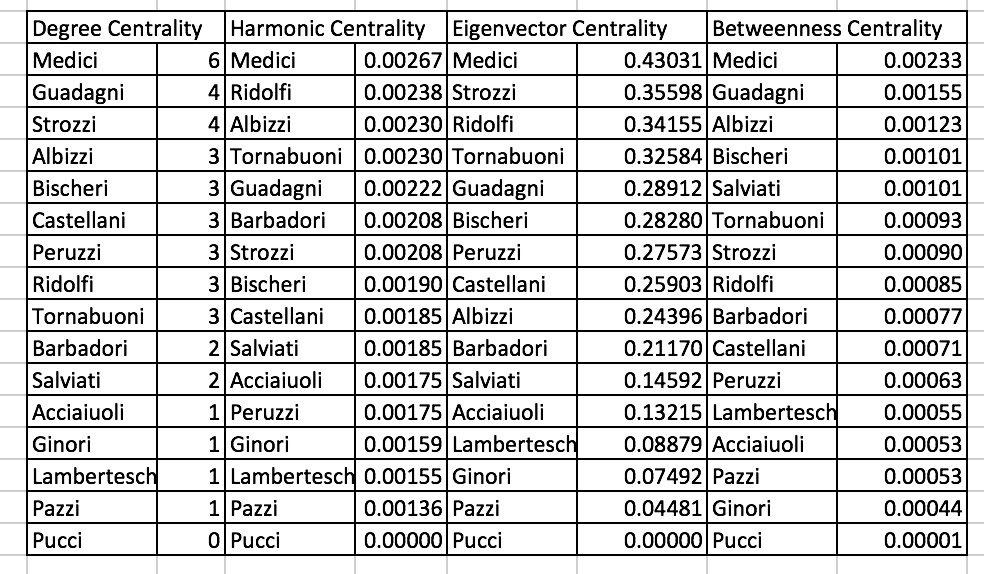
\includegraphics[scale = .9]{mediciTable}\\\\
\indent In all measures of centrality used, the Medici family emerges as the most central family(vertex) in the network of prominent 14th century Florentine families.This is in full agreement with the explanation for the Medici family's success, as given by Padgett and Andel in 1993.  What was unexpected, at least to me, was the variation in rank of the other families.  The Guadagni family was in the number two position in Degree and Betweenness centralities, but dropped to number five in both Harmonic and Eigenvector centralities, for example.  Many of the other families experienced radical changes in their positions, depending on the index used.   One possible explanation for this is the number of secondary hubs in the network.  The Ridolfi, Tornabuoni, and Strozzi families, among others, are all well-connected, with exact rankings varying by method used.\\\\\\
\includegraphics{picture1}\\
\indent While the Medici family's Harmonic Centrality score is approaching the 75th percentile, it is still within the 'norm' of 25th to 75th percentile, when compared to a run of 100,000 configuration models with identical degree sequence.  This would indicate that the Medici family, while having a high degree centrality score, is no more central to the network than should be expected.  The outliers in the harmonic centrality scores were the families connected to the Medici family.  Five of six of the Medici family's neighbors had harmonic centrality scores above the 75th percentile, as a result of the high centrality of the Medici family.  This may have been the key to the Medici family's success, not by being extremely central themselves, but by influencing the network in such a way that all of their neighbors were unusually well-connected.\\\\\\
6.a.\\
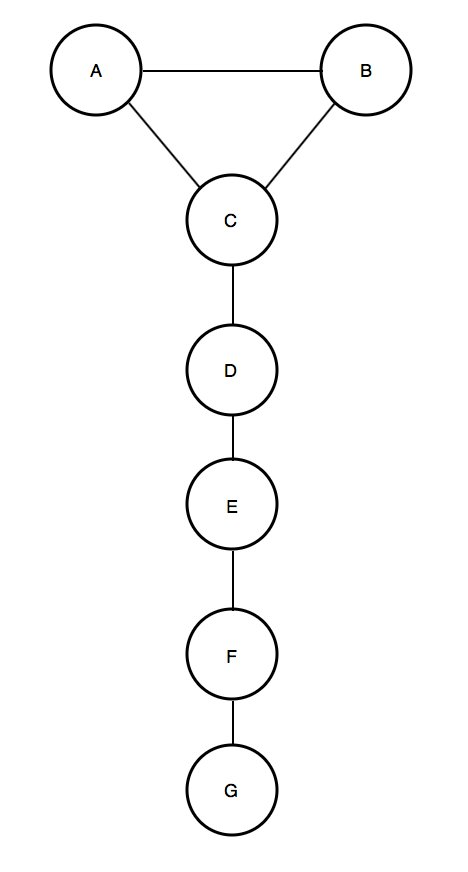
\includegraphics[scale=.5]{smallNetwork}
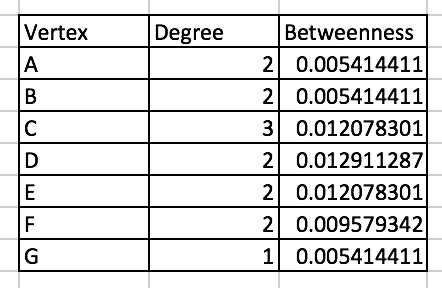
\includegraphics{smallTable}
\\\\
Vertex C has the highest degree, at 3, while vertex D has the highest betweenness, at 0.012911287.\\\\\\\\

\inputminted[linenos,fontsize=\scriptsize]{python}{medici.py}

\inputminted[linenos,fontsize=\scriptsize]{python}{smallGraph.py}

\end{document}  